\documentclass[1p]{elsarticle_modified}
%\bibliographystyle{elsarticle-num}

%\usepackage[colorlinks]{hyperref}
%\usepackage{abbrmath_seonhwa} %\Abb, \Ascr, \Acal ,\Abf, \Afrak
\usepackage{amsfonts}
\usepackage{amssymb}
\usepackage{amsmath}
\usepackage{amsthm}
\usepackage{scalefnt}
\usepackage{amsbsy}
\usepackage{kotex}
\usepackage{caption}
\usepackage{subfig}
\usepackage{color}
\usepackage{graphicx}
\usepackage{xcolor} %% white, black, red, green, blue, cyan, magenta, yellow
\usepackage{float}
\usepackage{setspace}
\usepackage{hyperref}

\usepackage{tikz}
\usetikzlibrary{arrows}

\usepackage{multirow}
\usepackage{array} % fixed length table
\usepackage{hhline}

%%%%%%%%%%%%%%%%%%%%%
\makeatletter
\renewcommand*\env@matrix[1][\arraystretch]{%
	\edef\arraystretch{#1}%
	\hskip -\arraycolsep
	\let\@ifnextchar\new@ifnextchar
	\array{*\c@MaxMatrixCols c}}
\makeatother %https://tex.stackexchange.com/questions/14071/how-can-i-increase-the-line-spacing-in-a-matrix
%%%%%%%%%%%%%%%

\usepackage[normalem]{ulem}

\newcommand{\msout}[1]{\ifmmode\text{\sout{\ensuremath{#1}}}\else\sout{#1}\fi}
%SOURCE: \msout is \stkout macro in https://tex.stackexchange.com/questions/20609/strikeout-in-math-mode

\newcommand{\cancel}[1]{
	\ifmmode
	{\color{red}\msout{#1}}
	\else
	{\color{red}\sout{#1}}
	\fi
}

\newcommand{\add}[1]{
	{\color{blue}\uwave{#1}}
}

\newcommand{\replace}[2]{
	\ifmmode
	{\color{red}\msout{#1}}{\color{blue}\uwave{#2}}
	\else
	{\color{red}\sout{#1}}{\color{blue}\uwave{#2}}
	\fi
}

\newcommand{\Sol}{\mathcal{S}} %segment
\newcommand{\D}{D} %diagram
\newcommand{\A}{\mathcal{A}} %arc


%%%%%%%%%%%%%%%%%%%%%%%%%%%%%5 test

\def\sl{\operatorname{\textup{SL}}(2,\Cbb)}
\def\psl{\operatorname{\textup{PSL}}(2,\Cbb)}
\def\quan{\mkern 1mu \triangleright \mkern 1mu}

\theoremstyle{definition}
\newtheorem{thm}{Theorem}[section]
\newtheorem{prop}[thm]{Proposition}
\newtheorem{lem}[thm]{Lemma}
\newtheorem{ques}[thm]{Question}
\newtheorem{cor}[thm]{Corollary}
\newtheorem{defn}[thm]{Definition}
\newtheorem{exam}[thm]{Example}
\newtheorem{rmk}[thm]{Remark}
\newtheorem{alg}[thm]{Algorithm}

\newcommand{\I}{\sqrt{-1}}
\begin{document}

%\begin{frontmatter}
%
%\title{Boundary parabolic representations of knots up to 8 crossings}
%
%%% Group authors per affiliation:
%\author{Yunhi Cho} 
%\address{Department of Mathematics, University of Seoul, Seoul, Korea}
%\ead{yhcho@uos.ac.kr}
%
%
%\author{Seonhwa Kim} %\fnref{s_kim}}
%\address{Center for Geometry and Physics, Institute for Basic Science, Pohang, 37673, Korea}
%\ead{ryeona17@ibs.re.kr}
%
%\author{Hyuk Kim}
%\address{Department of Mathematical Sciences, Seoul National University, Seoul 08826, Korea}
%\ead{hyukkim@snu.ac.kr}
%
%\author{Seokbeom Yoon}
%\address{Department of Mathematical Sciences, Seoul National University, Seoul, 08826,  Korea}
%\ead{sbyoon15@snu.ac.kr}
%
%\begin{abstract}
%We find all boundary parabolic representation of knots up to 8 crossings.
%
%\end{abstract}
%\begin{keyword}
%    \MSC[2010] 57M25 
%\end{keyword}
%
%\end{frontmatter}

%\linenumbers
%\tableofcontents
%
\newcommand\colored[1]{\textcolor{white}{\rule[-0.35ex]{0.8em}{1.4ex}}\kern-0.8em\color{red} #1}%
%\newcommand\colored[1]{\textcolor{white}{ #1}\kern-2.17ex	\textcolor{white}{ #1}\kern-1.81ex	\textcolor{white}{ #1}\kern-2.15ex\color{red}#1	}

{\Large $\underline{12a_{0356}~(K12a_{0356})}$}

\setlength{\tabcolsep}{10pt}
\renewcommand{\arraystretch}{1.6}
\vspace{1cm}\begin{tabular}{m{100pt}>{\centering\arraybackslash}m{274pt}}
\multirow{5}{120pt}{
	\centering
	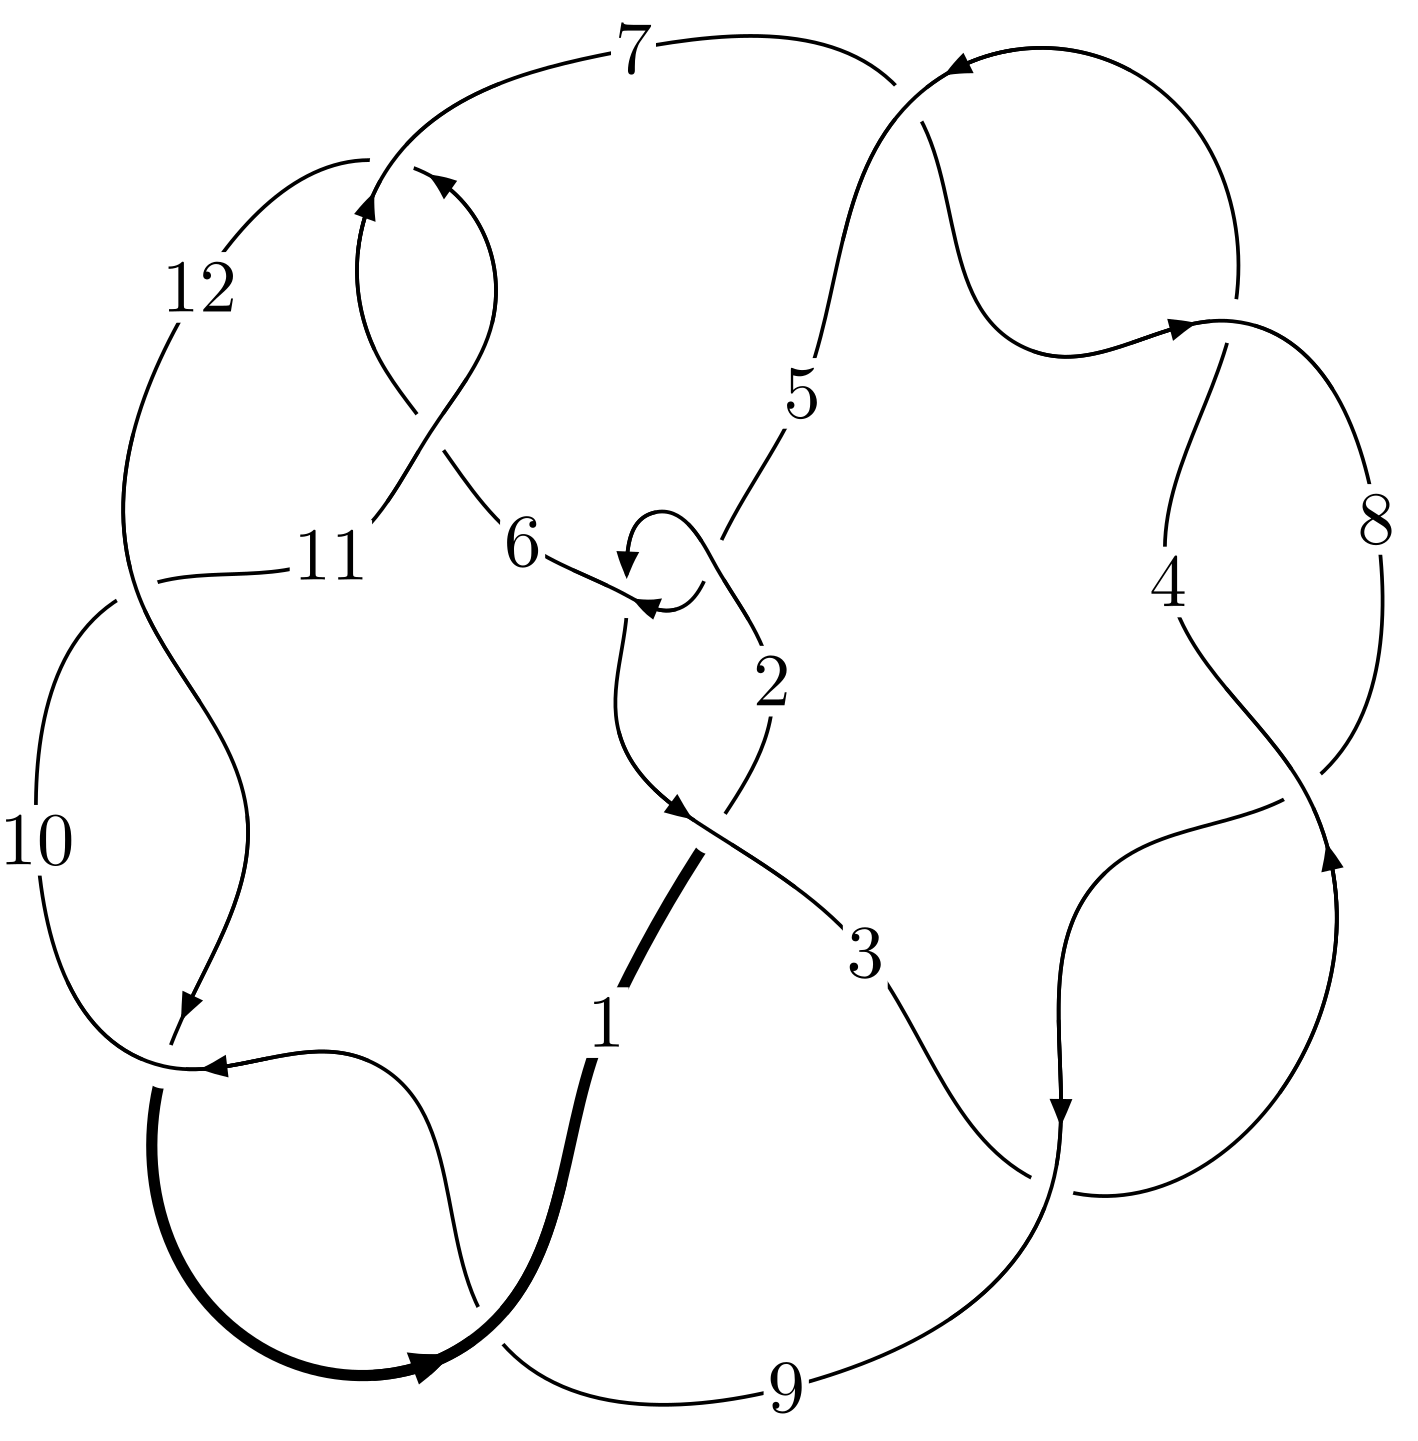
\includegraphics[width=112pt]{../../../GIT/diagram.site/Diagrams/png/1157_12a_0356.png}\\
\ \ \ A knot diagram\footnotemark}&
\allowdisplaybreaks
\textbf{Linearized knot diagam} \\
\cline{2-2}
 &
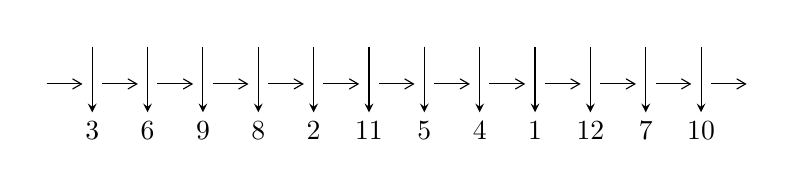
\begin{tikzpicture}[x=20pt, y=17pt]
	% nodes
	\node (C0) at (0, 0) {};
	\node (C1) at (1, 0) {};
	\node (C1U) at (1, +1) {};
	\node (C1D) at (1, -1) {3};

	\node (C2) at (2, 0) {};
	\node (C2U) at (2, +1) {};
	\node (C2D) at (2, -1) {6};

	\node (C3) at (3, 0) {};
	\node (C3U) at (3, +1) {};
	\node (C3D) at (3, -1) {9};

	\node (C4) at (4, 0) {};
	\node (C4U) at (4, +1) {};
	\node (C4D) at (4, -1) {8};

	\node (C5) at (5, 0) {};
	\node (C5U) at (5, +1) {};
	\node (C5D) at (5, -1) {2};

	\node (C6) at (6, 0) {};
	\node (C6U) at (6, +1) {};
	\node (C6D) at (6, -1) {11};

	\node (C7) at (7, 0) {};
	\node (C7U) at (7, +1) {};
	\node (C7D) at (7, -1) {5};

	\node (C8) at (8, 0) {};
	\node (C8U) at (8, +1) {};
	\node (C8D) at (8, -1) {4};

	\node (C9) at (9, 0) {};
	\node (C9U) at (9, +1) {};
	\node (C9D) at (9, -1) {1};

	\node (C10) at (10, 0) {};
	\node (C10U) at (10, +1) {};
	\node (C10D) at (10, -1) {12};

	\node (C11) at (11, 0) {};
	\node (C11U) at (11, +1) {};
	\node (C11D) at (11, -1) {7};

	\node (C12) at (12, 0) {};
	\node (C12U) at (12, +1) {};
	\node (C12D) at (12, -1) {10};
	\node (C13) at (13, 0) {};

	% arrows
	\draw[->,>={angle 60}]
	(C0) edge (C1) (C1) edge (C2) (C2) edge (C3) (C3) edge (C4) (C4) edge (C5) (C5) edge (C6) (C6) edge (C7) (C7) edge (C8) (C8) edge (C9) (C9) edge (C10) (C10) edge (C11) (C11) edge (C12) (C12) edge (C13) ;	\draw[->,>=stealth]
	(C1U) edge (C1D) (C2U) edge (C2D) (C3U) edge (C3D) (C4U) edge (C4D) (C5U) edge (C5D) (C6U) edge (C6D) (C7U) edge (C7D) (C8U) edge (C8D) (C9U) edge (C9D) (C10U) edge (C10D) (C11U) edge (C11D) (C12U) edge (C12D) ;
	\end{tikzpicture} \\
\hhline{~~} \\& 
\textbf{Solving Sequence} \\ \cline{2-2} 
 &
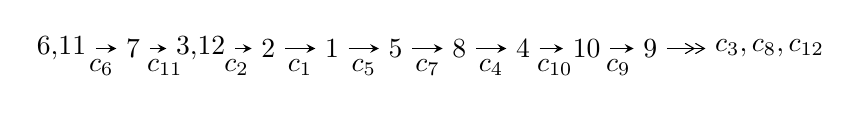
\begin{tikzpicture}[x=23pt, y=7pt]
	% node
	\node (A0) at (-1/8, 0) {6,11};
	\node (A1) at (1, 0) {7};
	\node (A2) at (33/16, 0) {3,12};
	\node (A3) at (25/8, 0) {2};
	\node (A4) at (33/8, 0) {1};
	\node (A5) at (41/8, 0) {5};
	\node (A6) at (49/8, 0) {8};
	\node (A7) at (57/8, 0) {4};
	\node (A8) at (65/8, 0) {10};
	\node (A9) at (73/8, 0) {9};
	\node (C1) at (1/2, -1) {$c_{6}$};
	\node (C2) at (3/2, -1) {$c_{11}$};
	\node (C3) at (21/8, -1) {$c_{2}$};
	\node (C4) at (29/8, -1) {$c_{1}$};
	\node (C5) at (37/8, -1) {$c_{5}$};
	\node (C6) at (45/8, -1) {$c_{7}$};
	\node (C7) at (53/8, -1) {$c_{4}$};
	\node (C8) at (61/8, -1) {$c_{10}$};
	\node (C9) at (69/8, -1) {$c_{9}$};
	\node (A10) at (11, 0) {$c_{3},c_{8},c_{12}$};

	% edge
	\draw[->,>=stealth]	
	(A0) edge (A1) (A1) edge (A2) (A2) edge (A3) (A3) edge (A4) (A4) edge (A5) (A5) edge (A6) (A6) edge (A7) (A7) edge (A8) (A8) edge (A9) ;
	\draw[->>,>={angle 60}]	
	(A9) edge (A10);
\end{tikzpicture} \\ 

\end{tabular} \\

\footnotetext{
The image of knot diagram is generated by the software ``\textbf{Draw programme}" developed by Andrew Bartholomew(\url{http://www.layer8.co.uk/maths/draw/index.htm\#Running-draw}), where we modified some parts for our purpose(\url{https://github.com/CATsTAILs/LinksPainter}).
}\phantom \\ \newline 
\centering \textbf{Ideals for irreducible components\footnotemark of $X_{\text{par}}$} 
 
\begin{align*}
I^u_{1}&=\langle 
-5.66231\times10^{18} u^{58}+4.32374\times10^{18} u^{57}+\cdots+8.19653\times10^{18} b+1.17819\times10^{19},\\
\phantom{I^u_{1}}&\phantom{= \langle  }7.79962\times10^{19} u^{58}-1.20924\times10^{20} u^{57}+\cdots+4.91792\times10^{19} a-4.08773\times10^{20},\;u^{59}-2 u^{58}+\cdots+u+3\rangle \\
I^u_{2}&=\langle 
b-1,\;a^2+2 a u+3 u^2-2 a-6 u+3,\;u^3- u^2+1\rangle \\
I^u_{3}&=\langle 
b+1,\;a+u+1,\;u^3+u^2-1\rangle \\
\\
\end{align*}
\raggedright * 3 irreducible components of $\dim_{\mathbb{C}}=0$, with total 68 representations.\\
\footnotetext{All coefficients of polynomials are rational numbers. But the coefficients are sometimes approximated in decimal forms when there is not enough margin.}
\newpage
\renewcommand{\arraystretch}{1}
\centering \section*{I. $I^u_{1}= \langle -5.66\times10^{18} u^{58}+4.32\times10^{18} u^{57}+\cdots+8.20\times10^{18} b+1.18\times10^{19},\;7.80\times10^{19} u^{58}-1.21\times10^{20} u^{57}+\cdots+4.92\times10^{19} a-4.09\times10^{20},\;u^{59}-2 u^{58}+\cdots+u+3 \rangle$}
\flushleft \textbf{(i) Arc colorings}\\
\begin{tabular}{m{7pt} m{180pt} m{7pt} m{180pt} }
\flushright $a_{6}=$&$\begin{pmatrix}1\\0\end{pmatrix}$ \\
\flushright $a_{11}=$&$\begin{pmatrix}0\\u\end{pmatrix}$ \\
\flushright $a_{7}=$&$\begin{pmatrix}1\\u^2\end{pmatrix}$ \\
\flushright $a_{3}=$&$\begin{pmatrix}-1.58596 u^{58}+2.45885 u^{57}+\cdots+9.55113 u+8.31191\\0.690818 u^{58}-0.527509 u^{57}+\cdots-0.607836 u-1.43742\end{pmatrix}$ \\
\flushright $a_{12}=$&$\begin{pmatrix}- u\\- u^3+u\end{pmatrix}$ \\
\flushright $a_{2}=$&$\begin{pmatrix}-0.895140 u^{58}+1.93134 u^{57}+\cdots+8.94330 u+6.87449\\0.690818 u^{58}-0.527509 u^{57}+\cdots-0.607836 u-1.43742\end{pmatrix}$ \\
\flushright $a_{1}=$&$\begin{pmatrix}- u^5- u\\- u^7+u^5-2 u^3+u\end{pmatrix}$ \\
\flushright $a_{5}=$&$\begin{pmatrix}1.92952 u^{58}-2.67059 u^{57}+\cdots-12.7404 u-7.85154\\-0.222016 u^{58}-0.0475838 u^{57}+\cdots+0.650562 u-0.281439\end{pmatrix}$ \\
\flushright $a_{8}=$&$\begin{pmatrix}1.18721 u^{58}-1.74998 u^{57}+\cdots+3.24272 u+0.910386\\0.412864 u^{58}-0.942970 u^{57}+\cdots-5.73768 u-1.86980\end{pmatrix}$ \\
\flushright $a_{4}=$&$\begin{pmatrix}-1.56955 u^{58}+2.85972 u^{57}+\cdots+12.4812 u+9.51305\\0.495410 u^{58}-0.282318 u^{57}+\cdots+1.25035 u-0.561736\end{pmatrix}$ \\
\flushright $a_{10}=$&$\begin{pmatrix}u^3\\u^5- u^3+u\end{pmatrix}$ \\
\flushright $a_{9}=$&$\begin{pmatrix}u^7+2 u^3\\u^9- u^7+3 u^5-2 u^3+u\end{pmatrix}$\\&\end{tabular}
\flushleft \textbf{(ii) Obstruction class $= -1$}\\~\\
\flushleft \textbf{(iii) Cusp Shapes $= \frac{23751865828353822111}{8196531629884877029} u^{58}-\frac{18808285269894389520}{8196531629884877029} u^{57}+\cdots-\frac{86244640466854553084}{8196531629884877029} u-\frac{226494452198725358175}{8196531629884877029}$}\\~\\
\newpage\renewcommand{\arraystretch}{1}
\flushleft \textbf{(iv) u-Polynomials at the component}\newline \\
\begin{tabular}{m{50pt}|m{274pt}}
Crossings & \hspace{64pt}u-Polynomials at each crossing \\
\hline $$\begin{aligned}c_{1}\end{aligned}$$&$\begin{aligned}
&u^{59}+24 u^{58}+\cdots-32 u+1
\end{aligned}$\\
\hline $$\begin{aligned}c_{2},c_{5}\end{aligned}$$&$\begin{aligned}
&u^{59}+4 u^{58}+\cdots-4 u+1
\end{aligned}$\\
\hline $$\begin{aligned}c_{3},c_{4},c_{7}\\c_{8}\end{aligned}$$&$\begin{aligned}
&u^{59}- u^{58}+\cdots+64 u^2+8
\end{aligned}$\\
\hline $$\begin{aligned}c_{6},c_{11}\end{aligned}$$&$\begin{aligned}
&u^{59}-2 u^{58}+\cdots+u+3
\end{aligned}$\\
\hline $$\begin{aligned}c_{9},c_{10},c_{12}\end{aligned}$$&$\begin{aligned}
&u^{59}+14 u^{58}+\cdots+157 u+9
\end{aligned}$\\
\hline
\end{tabular}\\~\\
\newpage\renewcommand{\arraystretch}{1}
\flushleft \textbf{(v) Riley Polynomials at the component}\newline \\
\begin{tabular}{m{50pt}|m{274pt}}
Crossings & \hspace{64pt}Riley Polynomials at each crossing \\
\hline $$\begin{aligned}c_{1}\end{aligned}$$&$\begin{aligned}
&y^{59}+32 y^{58}+\cdots-1936 y-1
\end{aligned}$\\
\hline $$\begin{aligned}c_{2},c_{5}\end{aligned}$$&$\begin{aligned}
&y^{59}-24 y^{58}+\cdots-32 y-1
\end{aligned}$\\
\hline $$\begin{aligned}c_{3},c_{4},c_{7}\\c_{8}\end{aligned}$$&$\begin{aligned}
&y^{59}+73 y^{58}+\cdots-1024 y-64
\end{aligned}$\\
\hline $$\begin{aligned}c_{6},c_{11}\end{aligned}$$&$\begin{aligned}
&y^{59}-14 y^{58}+\cdots+157 y-9
\end{aligned}$\\
\hline $$\begin{aligned}c_{9},c_{10},c_{12}\end{aligned}$$&$\begin{aligned}
&y^{59}+66 y^{58}+\cdots-1307 y-81
\end{aligned}$\\
\hline
\end{tabular}\\~\\
\newpage\flushleft \textbf{(vi) Complex Volumes and Cusp Shapes}
$$\begin{array}{c|c|c}  
\text{Solutions to }I^u_{1}& \I (\text{vol} + \sqrt{-1}CS) & \text{Cusp shape}\\
 \hline 
\begin{aligned}
u &= -0.950749 + 0.085534 I \\
a &= \phantom{-}1.40102 + 0.37767 I \\
b &= \phantom{-}0.881025 + 0.388729 I\end{aligned}
 & -2.20168 - 1.55351 I & -13.9942 + 4.5761 I \\ \hline\begin{aligned}
u &= -0.950749 - 0.085534 I \\
a &= \phantom{-}1.40102 - 0.37767 I \\
b &= \phantom{-}0.881025 - 0.388729 I\end{aligned}
 & -2.20168 + 1.55351 I & -13.9942 - 4.5761 I \\ \hline\begin{aligned}
u &= \phantom{-}0.955755 + 0.424887 I \\
a &= \phantom{-}1.39192 - 1.56772 I \\
b &= \phantom{-}1.001090 + 0.566158 I\end{aligned}
 & -0.26151 - 6.93624 I & -11.4611 + 10.0156 I \\ \hline\begin{aligned}
u &= \phantom{-}0.955755 - 0.424887 I \\
a &= \phantom{-}1.39192 + 1.56772 I \\
b &= \phantom{-}1.001090 - 0.566158 I\end{aligned}
 & -0.26151 + 6.93624 I & -11.4611 - 10.0156 I \\ \hline\begin{aligned}
u &= \phantom{-}1.061230 + 0.059722 I \\
a &= -1.249430 + 0.518825 I \\
b &= -0.871450 + 0.680013 I\end{aligned}
 & \phantom{-}5.44848 + 2.62573 I & -10.72193 - 2.36500 I \\ \hline\begin{aligned}
u &= \phantom{-}1.061230 - 0.059722 I \\
a &= -1.249430 - 0.518825 I \\
b &= -0.871450 - 0.680013 I\end{aligned}
 & \phantom{-}5.44848 - 2.62573 I & -10.72193 + 2.36500 I \\ \hline\begin{aligned}
u &= \phantom{-}0.808456 + 0.470326 I \\
a &= -0.499696 - 0.009506 I \\
b &= \phantom{-}0.399158 - 0.576724 I\end{aligned}
 & \phantom{-}1.30057 - 2.44037 I & -6.97566 + 5.43591 I \\ \hline\begin{aligned}
u &= \phantom{-}0.808456 - 0.470326 I \\
a &= -0.499696 + 0.009506 I \\
b &= \phantom{-}0.399158 + 0.576724 I\end{aligned}
 & \phantom{-}1.30057 + 2.44037 I & -6.97566 - 5.43591 I \\ \hline\begin{aligned}
u &= -0.841496 + 0.395242 I \\
a &= -0.96036 - 2.04635 I \\
b &= -0.942517 + 0.431284 I\end{aligned}
 & -1.79109 + 3.29910 I & -14.9386 - 5.3714 I \\ \hline\begin{aligned}
u &= -0.841496 - 0.395242 I \\
a &= -0.96036 + 2.04635 I \\
b &= -0.942517 - 0.431284 I\end{aligned}
 & -1.79109 - 3.29910 I & -14.9386 + 5.3714 I\\
 \hline 
 \end{array}$$\newpage$$\begin{array}{c|c|c}  
\text{Solutions to }I^u_{1}& \I (\text{vol} + \sqrt{-1}CS) & \text{Cusp shape}\\
 \hline 
\begin{aligned}
u &= -0.428912 + 0.779191 I \\
a &= \phantom{-}0.069578 - 1.101110 I \\
b &= -0.759172 + 0.857390 I\end{aligned}
 & \phantom{-}10.95100 + 1.36331 I & -3.49056 - 2.36160 I \\ \hline\begin{aligned}
u &= -0.428912 - 0.779191 I \\
a &= \phantom{-}0.069578 + 1.101110 I \\
b &= -0.759172 - 0.857390 I\end{aligned}
 & \phantom{-}10.95100 - 1.36331 I & -3.49056 + 2.36160 I \\ \hline\begin{aligned}
u &= -1.039320 + 0.443029 I \\
a &= -1.56082 - 1.25858 I \\
b &= -1.062320 + 0.707142 I\end{aligned}
 & \phantom{-}7.76213 + 9.14001 I & -12.0000 - 7.5958 I \\ \hline\begin{aligned}
u &= -1.039320 - 0.443029 I \\
a &= -1.56082 + 1.25858 I \\
b &= -1.062320 - 0.707142 I\end{aligned}
 & \phantom{-}7.76213 - 9.14001 I & -12.0000 + 7.5958 I \\ \hline\begin{aligned}
u &= \phantom{-}0.883608 + 0.704164 I \\
a &= \phantom{-}0.236690 - 0.559685 I \\
b &= \phantom{-}0.746146 - 0.071860 I\end{aligned}
 & \phantom{-}1.94353 - 2.69934 I & \phantom{-0.000000 } 0 \\ \hline\begin{aligned}
u &= \phantom{-}0.883608 - 0.704164 I \\
a &= \phantom{-}0.236690 + 0.559685 I \\
b &= \phantom{-}0.746146 + 0.071860 I\end{aligned}
 & \phantom{-}1.94353 + 2.69934 I & \phantom{-0.000000 } 0 \\ \hline\begin{aligned}
u &= -0.995779 + 0.541016 I \\
a &= \phantom{-}0.394659 - 0.390928 I \\
b &= -0.608688 - 0.798203 I\end{aligned}
 & \phantom{-}9.11589 + 3.43180 I & -12.00000 + 0. I\phantom{ +0.000000I} \\ \hline\begin{aligned}
u &= -0.995779 - 0.541016 I \\
a &= \phantom{-}0.394659 + 0.390928 I \\
b &= -0.608688 + 0.798203 I\end{aligned}
 & \phantom{-}9.11589 - 3.43180 I & -12.00000 + 0. I\phantom{ +0.000000I} \\ \hline\begin{aligned}
u &= -0.865723 + 0.753965 I \\
a &= -0.987861 + 0.232003 I \\
b &= \phantom{-}0.0644711 - 0.1218690 I\end{aligned}
 & \phantom{-}7.97460 + 2.84682 I & \phantom{-0.000000 } 0 \\ \hline\begin{aligned}
u &= -0.865723 - 0.753965 I \\
a &= -0.987861 - 0.232003 I \\
b &= \phantom{-}0.0644711 + 0.1218690 I\end{aligned}
 & \phantom{-}7.97460 - 2.84682 I & \phantom{-0.000000 } 0\\
 \hline 
 \end{array}$$\newpage$$\begin{array}{c|c|c}  
\text{Solutions to }I^u_{1}& \I (\text{vol} + \sqrt{-1}CS) & \text{Cusp shape}\\
 \hline 
\begin{aligned}
u &= -0.287017 + 0.779308 I \\
a &= \phantom{-}0.328056 + 0.939299 I \\
b &= -0.992597 - 0.783531 I\end{aligned}
 & \phantom{-}10.23980 - 4.73907 I & -4.25165 + 2.78795 I \\ \hline\begin{aligned}
u &= -0.287017 - 0.779308 I \\
a &= \phantom{-}0.328056 - 0.939299 I \\
b &= -0.992597 + 0.783531 I\end{aligned}
 & \phantom{-}10.23980 + 4.73907 I & -4.25165 - 2.78795 I \\ \hline\begin{aligned}
u &= -0.718782 + 0.401065 I \\
a &= \phantom{-}1.86408 + 0.41857 I \\
b &= \phantom{-}1.231790 + 0.111942 I\end{aligned}
 & \phantom{-}3.40228 + 1.59157 I & -9.70315 - 4.05404 I \\ \hline\begin{aligned}
u &= -0.718782 - 0.401065 I \\
a &= \phantom{-}1.86408 - 0.41857 I \\
b &= \phantom{-}1.231790 - 0.111942 I\end{aligned}
 & \phantom{-}3.40228 - 1.59157 I & -9.70315 + 4.05404 I \\ \hline\begin{aligned}
u &= \phantom{-}0.779291 + 0.186002 I \\
a &= -1.76043 + 0.35358 I \\
b &= -1.092770 + 0.150850 I\end{aligned}
 & -2.95013 - 0.58618 I & -15.2527 + 9.8012 I \\ \hline\begin{aligned}
u &= \phantom{-}0.779291 - 0.186002 I \\
a &= -1.76043 - 0.35358 I \\
b &= -1.092770 - 0.150850 I\end{aligned}
 & -2.95013 + 0.58618 I & -15.2527 - 9.8012 I \\ \hline\begin{aligned}
u &= -0.893562 + 0.803723 I \\
a &= -0.002799 - 0.814217 I \\
b &= -1.251010 - 0.015615 I\end{aligned}
 & \phantom{-}2.63289 + 3.01191 I & \phantom{-0.000000 } 0 \\ \hline\begin{aligned}
u &= -0.893562 - 0.803723 I \\
a &= -0.002799 + 0.814217 I \\
b &= -1.251010 + 0.015615 I\end{aligned}
 & \phantom{-}2.63289 - 3.01191 I & \phantom{-0.000000 } 0 \\ \hline\begin{aligned}
u &= -0.854945 + 0.893449 I \\
a &= -0.723640 - 1.049790 I \\
b &= \phantom{-}1.036460 + 0.751160 I\end{aligned}
 & \phantom{-}8.28053 - 4.23254 I & \phantom{-0.000000 } 0 \\ \hline\begin{aligned}
u &= -0.854945 - 0.893449 I \\
a &= -0.723640 + 1.049790 I \\
b &= \phantom{-}1.036460 - 0.751160 I\end{aligned}
 & \phantom{-}8.28053 + 4.23254 I & \phantom{-0.000000 } 0\\
 \hline 
 \end{array}$$\newpage$$\begin{array}{c|c|c}  
\text{Solutions to }I^u_{1}& \I (\text{vol} + \sqrt{-1}CS) & \text{Cusp shape}\\
 \hline 
\begin{aligned}
u &= \phantom{-}0.886324 + 0.866549 I \\
a &= \phantom{-}0.98642 - 1.06679 I \\
b &= -0.845945 + 0.735665 I\end{aligned}
 & \phantom{-}5.94223 - 0.39886 I & \phantom{-0.000000 } 0 \\ \hline\begin{aligned}
u &= \phantom{-}0.886324 - 0.866549 I \\
a &= \phantom{-}0.98642 + 1.06679 I \\
b &= -0.845945 - 0.735665 I\end{aligned}
 & \phantom{-}5.94223 + 0.39886 I & \phantom{-0.000000 } 0 \\ \hline\begin{aligned}
u &= \phantom{-}0.832835 + 0.926311 I \\
a &= \phantom{-}0.571242 - 0.903844 I \\
b &= -1.18749 + 0.79875 I\end{aligned}
 & \phantom{-}16.9600 + 7.2294 I & \phantom{-0.000000 } 0 \\ \hline\begin{aligned}
u &= \phantom{-}0.832835 - 0.926311 I \\
a &= \phantom{-}0.571242 + 0.903844 I \\
b &= -1.18749 - 0.79875 I\end{aligned}
 & \phantom{-}16.9600 - 7.2294 I & \phantom{-0.000000 } 0 \\ \hline\begin{aligned}
u &= -0.897663 + 0.871706 I \\
a &= -0.13642 + 1.69360 I \\
b &= \phantom{-}0.673711 - 0.844140 I\end{aligned}
 & \phantom{-}9.36550 + 1.73164 I & \phantom{-0.000000 } 0 \\ \hline\begin{aligned}
u &= -0.897663 - 0.871706 I \\
a &= -0.13642 - 1.69360 I \\
b &= \phantom{-}0.673711 + 0.844140 I\end{aligned}
 & \phantom{-}9.36550 - 1.73164 I & \phantom{-0.000000 } 0 \\ \hline\begin{aligned}
u &= \phantom{-}0.915394 + 0.861826 I \\
a &= -0.067431 - 0.859114 I \\
b &= \phantom{-}1.48127 - 0.02057 I\end{aligned}
 & \phantom{-}10.78160 - 3.19575 I & \phantom{-0.000000 } 0 \\ \hline\begin{aligned}
u &= \phantom{-}0.915394 - 0.861826 I \\
a &= -0.067431 + 0.859114 I \\
b &= \phantom{-}1.48127 + 0.02057 I\end{aligned}
 & \phantom{-}10.78160 + 3.19575 I & \phantom{-0.000000 } 0 \\ \hline\begin{aligned}
u &= \phantom{-}0.938182 + 0.846227 I \\
a &= \phantom{-}0.00707 + 2.10628 I \\
b &= -0.898285 - 0.723052 I\end{aligned}
 & \phantom{-}5.77879 - 5.95695 I & \phantom{-0.000000 } 0 \\ \hline\begin{aligned}
u &= \phantom{-}0.938182 - 0.846227 I \\
a &= \phantom{-}0.00707 - 2.10628 I \\
b &= -0.898285 + 0.723052 I\end{aligned}
 & \phantom{-}5.77879 + 5.95695 I & \phantom{-0.000000 } 0\\
 \hline 
 \end{array}$$\newpage$$\begin{array}{c|c|c}  
\text{Solutions to }I^u_{1}& \I (\text{vol} + \sqrt{-1}CS) & \text{Cusp shape}\\
 \hline 
\begin{aligned}
u &= -0.933873 + 0.857641 I \\
a &= -1.114390 - 0.849709 I \\
b &= \phantom{-}0.624353 + 0.869336 I\end{aligned}
 & \phantom{-}9.25182 + 4.67664 I & \phantom{-0.000000 } 0 \\ \hline\begin{aligned}
u &= -0.933873 - 0.857641 I \\
a &= -1.114390 + 0.849709 I \\
b &= \phantom{-}0.624353 - 0.869336 I\end{aligned}
 & \phantom{-}9.25182 - 4.67664 I & \phantom{-0.000000 } 0 \\ \hline\begin{aligned}
u &= \phantom{-}0.875079 + 0.923683 I \\
a &= -0.06377 + 1.45605 I \\
b &= -0.571370 - 1.103440 I\end{aligned}
 & \phantom{-}18.8901 + 0.4011 I & \phantom{-0.000000 } 0 \\ \hline\begin{aligned}
u &= \phantom{-}0.875079 - 0.923683 I \\
a &= -0.06377 - 1.45605 I \\
b &= -0.571370 + 1.103440 I\end{aligned}
 & \phantom{-}18.8901 - 0.4011 I & \phantom{-0.000000 } 0 \\ \hline\begin{aligned}
u &= \phantom{-}0.469446 + 0.544141 I \\
a &= -0.223809 - 1.235640 I \\
b &= \phantom{-}0.654076 + 0.529004 I\end{aligned}
 & \phantom{-}2.26071 - 1.37979 I & -4.27858 + 3.91647 I \\ \hline\begin{aligned}
u &= \phantom{-}0.469446 - 0.544141 I \\
a &= -0.223809 + 1.235640 I \\
b &= \phantom{-}0.654076 - 0.529004 I\end{aligned}
 & \phantom{-}2.26071 + 1.37979 I & -4.27858 - 3.91647 I \\ \hline\begin{aligned}
u &= \phantom{-}0.667363 + 0.266454 I \\
a &= -0.70482 - 2.96122 I \\
b &= \phantom{-}0.852790 + 0.242476 I\end{aligned}
 & \phantom{-}2.81040 - 1.03770 I & -8.02636 + 6.84259 I \\ \hline\begin{aligned}
u &= \phantom{-}0.667363 - 0.266454 I \\
a &= -0.70482 + 2.96122 I \\
b &= \phantom{-}0.852790 - 0.242476 I\end{aligned}
 & \phantom{-}2.81040 + 1.03770 I & -8.02636 - 6.84259 I \\ \hline\begin{aligned}
u &= -0.972360 + 0.842990 I \\
a &= \phantom{-}0.31648 + 2.17743 I \\
b &= \phantom{-}1.070130 - 0.736498 I\end{aligned}
 & \phantom{-}7.90798 + 10.65770 I & \phantom{-0.000000 } 0 \\ \hline\begin{aligned}
u &= -0.972360 - 0.842990 I \\
a &= \phantom{-}0.31648 - 2.17743 I \\
b &= \phantom{-}1.070130 + 0.736498 I\end{aligned}
 & \phantom{-}7.90798 - 10.65770 I & \phantom{-0.000000 } 0\\
 \hline 
 \end{array}$$\newpage$$\begin{array}{c|c|c}  
\text{Solutions to }I^u_{1}& \I (\text{vol} + \sqrt{-1}CS) & \text{Cusp shape}\\
 \hline 
\begin{aligned}
u &= \phantom{-}0.312980 + 0.623983 I \\
a &= -0.499965 + 1.002160 I \\
b &= \phantom{-}0.872314 - 0.581880 I\end{aligned}
 & \phantom{-}1.73082 + 3.05513 I & -5.72428 - 4.49353 I \\ \hline\begin{aligned}
u &= \phantom{-}0.312980 - 0.623983 I \\
a &= -0.499965 - 1.002160 I \\
b &= \phantom{-}0.872314 + 0.581880 I\end{aligned}
 & \phantom{-}1.73082 - 3.05513 I & -5.72428 + 4.49353 I \\ \hline\begin{aligned}
u &= \phantom{-}1.002690 + 0.845529 I \\
a &= -0.53525 + 2.09749 I \\
b &= -1.20584 - 0.77319 I\end{aligned}
 & \phantom{-}16.4153 - 13.7600 I & \phantom{-0.000000 } 0 \\ \hline\begin{aligned}
u &= \phantom{-}1.002690 - 0.845529 I \\
a &= -0.53525 - 2.09749 I \\
b &= -1.20584 + 0.77319 I\end{aligned}
 & \phantom{-}16.4153 + 13.7600 I & \phantom{-0.000000 } 0 \\ \hline\begin{aligned}
u &= \phantom{-}0.980128 + 0.871697 I \\
a &= \phantom{-}1.090820 - 0.722028 I \\
b &= -0.524644 + 1.106680 I\end{aligned}
 & \phantom{-}18.5511 - 7.0143 I & \phantom{-0.000000 } 0 \\ \hline\begin{aligned}
u &= \phantom{-}0.980128 - 0.871697 I \\
a &= \phantom{-}1.090820 + 0.722028 I \\
b &= -0.524644 - 1.106680 I\end{aligned}
 & \phantom{-}18.5511 + 7.0143 I & \phantom{-0.000000 } 0 \\ \hline\begin{aligned}
u &= -0.450920 + 0.353539 I \\
a &= \phantom{-}1.152780 + 0.540477 I \\
b &= -0.620312 - 0.297342 I\end{aligned}
 & -0.634650 - 0.118465 I & -11.69433 - 0.33232 I \\ \hline\begin{aligned}
u &= -0.450920 - 0.353539 I \\
a &= \phantom{-}1.152780 - 0.540477 I \\
b &= -0.620312 + 0.297342 I\end{aligned}
 & -0.634650 + 0.118465 I & -11.69433 + 0.33232 I \\ \hline\begin{aligned}
u &= -0.475308\phantom{ +0.000000I} \\
a &= \phantom{-}0.893509\phantom{ +0.000000I} \\
b &= -0.308761\phantom{ +0.000000I}\end{aligned}
 & -0.673099\phantom{ +0.000000I} & -14.6220\phantom{ +0.000000I}\\
 \hline 
 \end{array}$$\newpage\newpage\renewcommand{\arraystretch}{1}
\centering \section*{II. $I^u_{2}= \langle b-1,\;a^2+2 a u+3 u^2-2 a-6 u+3,\;u^3- u^2+1 \rangle$}
\flushleft \textbf{(i) Arc colorings}\\
\begin{tabular}{m{7pt} m{180pt} m{7pt} m{180pt} }
\flushright $a_{6}=$&$\begin{pmatrix}1\\0\end{pmatrix}$ \\
\flushright $a_{11}=$&$\begin{pmatrix}0\\u\end{pmatrix}$ \\
\flushright $a_{7}=$&$\begin{pmatrix}1\\u^2\end{pmatrix}$ \\
\flushright $a_{3}=$&$\begin{pmatrix}a\\1\end{pmatrix}$ \\
\flushright $a_{12}=$&$\begin{pmatrix}- u\\- u^2+u+1\end{pmatrix}$ \\
\flushright $a_{2}=$&$\begin{pmatrix}a+1\\1\end{pmatrix}$ \\
\flushright $a_{1}=$&$\begin{pmatrix}1\\0\end{pmatrix}$ \\
\flushright $a_{5}=$&$\begin{pmatrix}- a\\-1\end{pmatrix}$ \\
\flushright $a_{8}=$&$\begin{pmatrix}- a-3 u+4\\- u^2 a+u^2+1\end{pmatrix}$ \\
\flushright $a_{4}=$&$\begin{pmatrix}u^2 a+a-1\\u^2 a- a u- u^2- a+1\end{pmatrix}$ \\
\flushright $a_{10}=$&$\begin{pmatrix}u^2-1\\- u^2\end{pmatrix}$ \\
\flushright $a_{9}=$&$\begin{pmatrix}-1\\- u^2\end{pmatrix}$\\&\end{tabular}
\flushleft \textbf{(ii) Obstruction class $= 1$}\\~\\
\flushleft \textbf{(iii) Cusp Shapes $= 4 u-12$}\\~\\
\newpage\renewcommand{\arraystretch}{1}
\flushleft \textbf{(iv) u-Polynomials at the component}\newline \\
\begin{tabular}{m{50pt}|m{274pt}}
Crossings & \hspace{64pt}u-Polynomials at each crossing \\
\hline $$\begin{aligned}c_{1},c_{5}\end{aligned}$$&$\begin{aligned}
&(u-1)^6
\end{aligned}$\\
\hline $$\begin{aligned}c_{2}\end{aligned}$$&$\begin{aligned}
&(u+1)^6
\end{aligned}$\\
\hline $$\begin{aligned}c_{3},c_{4},c_{7}\\c_{8}\end{aligned}$$&$\begin{aligned}
&(u^2+2)^3
\end{aligned}$\\
\hline $$\begin{aligned}c_{6}\end{aligned}$$&$\begin{aligned}
&(u^3- u^2+1)^2
\end{aligned}$\\
\hline $$\begin{aligned}c_{9},c_{10}\end{aligned}$$&$\begin{aligned}
&(u^3- u^2+2 u-1)^2
\end{aligned}$\\
\hline $$\begin{aligned}c_{11}\end{aligned}$$&$\begin{aligned}
&(u^3+u^2-1)^2
\end{aligned}$\\
\hline $$\begin{aligned}c_{12}\end{aligned}$$&$\begin{aligned}
&(u^3+u^2+2 u+1)^2
\end{aligned}$\\
\hline
\end{tabular}\\~\\
\newpage\renewcommand{\arraystretch}{1}
\flushleft \textbf{(v) Riley Polynomials at the component}\newline \\
\begin{tabular}{m{50pt}|m{274pt}}
Crossings & \hspace{64pt}Riley Polynomials at each crossing \\
\hline $$\begin{aligned}c_{1},c_{2},c_{5}\end{aligned}$$&$\begin{aligned}
&(y-1)^6
\end{aligned}$\\
\hline $$\begin{aligned}c_{3},c_{4},c_{7}\\c_{8}\end{aligned}$$&$\begin{aligned}
&(y+2)^6
\end{aligned}$\\
\hline $$\begin{aligned}c_{6},c_{11}\end{aligned}$$&$\begin{aligned}
&(y^3- y^2+2 y-1)^2
\end{aligned}$\\
\hline $$\begin{aligned}c_{9},c_{10},c_{12}\end{aligned}$$&$\begin{aligned}
&(y^3+3 y^2+2 y-1)^2
\end{aligned}$\\
\hline
\end{tabular}\\~\\
\newpage\flushleft \textbf{(vi) Complex Volumes and Cusp Shapes}
$$\begin{array}{c|c|c}  
\text{Solutions to }I^u_{2}& \I (\text{vol} + \sqrt{-1}CS) & \text{Cusp shape}\\
 \hline 
\begin{aligned}
u &= \phantom{-}0.877439 + 0.744862 I \\
a &= \phantom{-}1.175960 - 0.571534 I \\
b &= \phantom{-}1.00000\phantom{ +0.000000I}\end{aligned}
 & \phantom{-}6.31400 - 2.82812 I & -8.49024 + 2.97945 I \\ \hline\begin{aligned}
u &= \phantom{-}0.877439 + 0.744862 I \\
a &= -0.930832 - 0.918189 I \\
b &= \phantom{-}1.00000\phantom{ +0.000000I}\end{aligned}
 & \phantom{-}6.31400 - 2.82812 I & -8.49024 + 2.97945 I \\ \hline\begin{aligned}
u &= \phantom{-}0.877439 - 0.744862 I \\
a &= \phantom{-}1.175960 + 0.571534 I \\
b &= \phantom{-}1.00000\phantom{ +0.000000I}\end{aligned}
 & \phantom{-}6.31400 + 2.82812 I & -8.49024 - 2.97945 I \\ \hline\begin{aligned}
u &= \phantom{-}0.877439 - 0.744862 I \\
a &= -0.930832 + 0.918189 I \\
b &= \phantom{-}1.00000\phantom{ +0.000000I}\end{aligned}
 & \phantom{-}6.31400 + 2.82812 I & -8.49024 - 2.97945 I \\ \hline\begin{aligned}
u &= -0.754878\phantom{ +0.000000I} \\
a &= \phantom{-}1.75488 + 2.48177 I \\
b &= \phantom{-}1.00000\phantom{ +0.000000I}\end{aligned}
 & \phantom{-}2.17641\phantom{ +0.000000I} & -15.0200\phantom{ +0.000000I} \\ \hline\begin{aligned}
u &= -0.754878\phantom{ +0.000000I} \\
a &= \phantom{-}1.75488 - 2.48177 I \\
b &= \phantom{-}1.00000\phantom{ +0.000000I}\end{aligned}
 & \phantom{-}2.17641\phantom{ +0.000000I} & -15.0200\phantom{ +0.000000I}\\
 \hline 
 \end{array}$$\newpage\newpage\renewcommand{\arraystretch}{1}
\centering \section*{III. $I^u_{3}= \langle b+1,\;a+u+1,\;u^3+u^2-1 \rangle$}
\flushleft \textbf{(i) Arc colorings}\\
\begin{tabular}{m{7pt} m{180pt} m{7pt} m{180pt} }
\flushright $a_{6}=$&$\begin{pmatrix}1\\0\end{pmatrix}$ \\
\flushright $a_{11}=$&$\begin{pmatrix}0\\u\end{pmatrix}$ \\
\flushright $a_{7}=$&$\begin{pmatrix}1\\u^2\end{pmatrix}$ \\
\flushright $a_{3}=$&$\begin{pmatrix}- u-1\\-1\end{pmatrix}$ \\
\flushright $a_{12}=$&$\begin{pmatrix}- u\\u^2+u-1\end{pmatrix}$ \\
\flushright $a_{2}=$&$\begin{pmatrix}- u-2\\-1\end{pmatrix}$ \\
\flushright $a_{1}=$&$\begin{pmatrix}-1\\0\end{pmatrix}$ \\
\flushright $a_{5}=$&$\begin{pmatrix}- u-1\\-1\end{pmatrix}$ \\
\flushright $a_{8}=$&$\begin{pmatrix}1\\u^2\end{pmatrix}$ \\
\flushright $a_{4}=$&$\begin{pmatrix}- u-1\\-1\end{pmatrix}$ \\
\flushright $a_{10}=$&$\begin{pmatrix}- u^2+1\\u^2\end{pmatrix}$ \\
\flushright $a_{9}=$&$\begin{pmatrix}1\\u^2\end{pmatrix}$\\&\end{tabular}
\flushleft \textbf{(ii) Obstruction class $= 1$}\\~\\
\flushleft \textbf{(iii) Cusp Shapes $= 4 u^2+2 u-16$}\\~\\
\newpage\renewcommand{\arraystretch}{1}
\flushleft \textbf{(iv) u-Polynomials at the component}\newline \\
\begin{tabular}{m{50pt}|m{274pt}}
Crossings & \hspace{64pt}u-Polynomials at each crossing \\
\hline $$\begin{aligned}c_{1},c_{2}\end{aligned}$$&$\begin{aligned}
&(u-1)^3
\end{aligned}$\\
\hline $$\begin{aligned}c_{3},c_{4},c_{7}\\c_{8}\end{aligned}$$&$\begin{aligned}
&u^3
\end{aligned}$\\
\hline $$\begin{aligned}c_{5}\end{aligned}$$&$\begin{aligned}
&(u+1)^3
\end{aligned}$\\
\hline $$\begin{aligned}c_{6}\end{aligned}$$&$\begin{aligned}
&u^3+u^2-1
\end{aligned}$\\
\hline $$\begin{aligned}c_{9},c_{10}\end{aligned}$$&$\begin{aligned}
&u^3- u^2+2 u-1
\end{aligned}$\\
\hline $$\begin{aligned}c_{11}\end{aligned}$$&$\begin{aligned}
&u^3- u^2+1
\end{aligned}$\\
\hline $$\begin{aligned}c_{12}\end{aligned}$$&$\begin{aligned}
&u^3+u^2+2 u+1
\end{aligned}$\\
\hline
\end{tabular}\\~\\
\newpage\renewcommand{\arraystretch}{1}
\flushleft \textbf{(v) Riley Polynomials at the component}\newline \\
\begin{tabular}{m{50pt}|m{274pt}}
Crossings & \hspace{64pt}Riley Polynomials at each crossing \\
\hline $$\begin{aligned}c_{1},c_{2},c_{5}\end{aligned}$$&$\begin{aligned}
&(y-1)^3
\end{aligned}$\\
\hline $$\begin{aligned}c_{3},c_{4},c_{7}\\c_{8}\end{aligned}$$&$\begin{aligned}
&y^3
\end{aligned}$\\
\hline $$\begin{aligned}c_{6},c_{11}\end{aligned}$$&$\begin{aligned}
&y^3- y^2+2 y-1
\end{aligned}$\\
\hline $$\begin{aligned}c_{9},c_{10},c_{12}\end{aligned}$$&$\begin{aligned}
&y^3+3 y^2+2 y-1
\end{aligned}$\\
\hline
\end{tabular}\\~\\
\newpage\flushleft \textbf{(vi) Complex Volumes and Cusp Shapes}
$$\begin{array}{c|c|c}  
\text{Solutions to }I^u_{3}& \I (\text{vol} + \sqrt{-1}CS) & \text{Cusp shape}\\
 \hline 
\begin{aligned}
u &= -0.877439 + 0.744862 I \\
a &= -0.122561 - 0.744862 I \\
b &= -1.00000\phantom{ +0.000000I}\end{aligned}
 & \phantom{-}1.37919 + 2.82812 I & -16.8946 - 3.7388 I \\ \hline\begin{aligned}
u &= -0.877439 - 0.744862 I \\
a &= -0.122561 + 0.744862 I \\
b &= -1.00000\phantom{ +0.000000I}\end{aligned}
 & \phantom{-}1.37919 - 2.82812 I & -16.8946 + 3.7388 I \\ \hline\begin{aligned}
u &= \phantom{-}0.754878\phantom{ +0.000000I} \\
a &= -1.75488\phantom{ +0.000000I} \\
b &= -1.00000\phantom{ +0.000000I}\end{aligned}
 & -2.75839\phantom{ +0.000000I} & -12.2110\phantom{ +0.000000I}\\
 \hline 
 \end{array}$$\newpage
\newpage\renewcommand{\arraystretch}{1}
\centering \section*{ IV. u-Polynomials}
\begin{tabular}{m{50pt}|m{274pt}}
Crossings & \hspace{64pt}u-Polynomials at each crossing \\
\hline $$\begin{aligned}c_{1}\end{aligned}$$&$\begin{aligned}
&((u-1)^9)(u^{59}+24 u^{58}+\cdots-32 u+1)
\end{aligned}$\\
\hline $$\begin{aligned}c_{2}\end{aligned}$$&$\begin{aligned}
&((u-1)^3)(u+1)^6(u^{59}+4 u^{58}+\cdots-4 u+1)
\end{aligned}$\\
\hline $$\begin{aligned}c_{3},c_{4},c_{7}\\c_{8}\end{aligned}$$&$\begin{aligned}
&u^3(u^2+2)^3(u^{59}- u^{58}+\cdots+64 u^2+8)
\end{aligned}$\\
\hline $$\begin{aligned}c_{5}\end{aligned}$$&$\begin{aligned}
&((u-1)^6)(u+1)^3(u^{59}+4 u^{58}+\cdots-4 u+1)
\end{aligned}$\\
\hline $$\begin{aligned}c_{6}\end{aligned}$$&$\begin{aligned}
&((u^3- u^2+1)^2)(u^3+u^2-1)(u^{59}-2 u^{58}+\cdots+u+3)
\end{aligned}$\\
\hline $$\begin{aligned}c_{9},c_{10}\end{aligned}$$&$\begin{aligned}
&((u^3- u^2+2 u-1)^3)(u^{59}+14 u^{58}+\cdots+157 u+9)
\end{aligned}$\\
\hline $$\begin{aligned}c_{11}\end{aligned}$$&$\begin{aligned}
&(u^3- u^2+1)(u^3+u^2-1)^2(u^{59}-2 u^{58}+\cdots+u+3)
\end{aligned}$\\
\hline $$\begin{aligned}c_{12}\end{aligned}$$&$\begin{aligned}
&((u^3+u^2+2 u+1)^3)(u^{59}+14 u^{58}+\cdots+157 u+9)
\end{aligned}$\\
\hline
\end{tabular}\newpage\renewcommand{\arraystretch}{1}
\centering \section*{ V. Riley Polynomials}
\begin{tabular}{m{50pt}|m{274pt}}
Crossings & \hspace{64pt}Riley Polynomials at each crossing \\
\hline $$\begin{aligned}c_{1}\end{aligned}$$&$\begin{aligned}
&((y-1)^9)(y^{59}+32 y^{58}+\cdots-1936 y-1)
\end{aligned}$\\
\hline $$\begin{aligned}c_{2},c_{5}\end{aligned}$$&$\begin{aligned}
&((y-1)^9)(y^{59}-24 y^{58}+\cdots-32 y-1)
\end{aligned}$\\
\hline $$\begin{aligned}c_{3},c_{4},c_{7}\\c_{8}\end{aligned}$$&$\begin{aligned}
&y^3(y+2)^6(y^{59}+73 y^{58}+\cdots-1024 y-64)
\end{aligned}$\\
\hline $$\begin{aligned}c_{6},c_{11}\end{aligned}$$&$\begin{aligned}
&((y^3- y^2+2 y-1)^3)(y^{59}-14 y^{58}+\cdots+157 y-9)
\end{aligned}$\\
\hline $$\begin{aligned}c_{9},c_{10},c_{12}\end{aligned}$$&$\begin{aligned}
&((y^3+3 y^2+2 y-1)^3)(y^{59}+66 y^{58}+\cdots-1307 y-81)
\end{aligned}$\\
\hline
\end{tabular}
\vskip 2pc
\end{document}